\clearpage

\begin{usecase}
    \addheading{Use-Case Description}
    \addsingletwocolumnrow{Name}{ugMonitor}
    \addsingletwocolumnrow{Scope}{System}
    \addsingletwocolumnrow{Altitude}{Summary}
    \addrowheading{Parameters}
    \addnumberedsinglerow{}{none}
    \addrowheading{Primary actor(s)}
    \addnumberedsinglerow{}{\msrcode{actCoordinator[active]}}
    \addnumberedsinglerow{}{\msrcode{actDomainExpert[active]}}
    \addrowheading{Secondary actor(s)}
    \addnumberedsinglerow{}{None.}
    \addrowheading{Goal(s) description}
    \addsinglerow{The goal is to use all operations available to the coordinator for the successful handling of a crisis or an alert received by our system.}
    \addrowheading{Reuse}
    \addnumberedsinglerow{}{\msrucname{oeGetAlertSet}}
    \addnumberedsinglerow{}{\msrucname{oeValidateAlert}}
    \addnumberedsinglerow{}{\msrucname{oeSollicitateCrisisHandling}}
    \addrowheading{Protocol condition(s)}
    \addnumberedsinglerow{}{the \msricrash system has been started}
    \addnumberedsinglerow{}{the \msrcode{actCoordinator} has been added to the system.}
    \addnumberedsinglerow{}{the \msrcode{actCoordinator} has safely logged on to the system.}
    \addnumberedsinglerow{}{the \msrcode{actDomainExpert} has safely logged on to system.}
    \addrowheading{Pre-condition(s)}
    \addnumberedsinglerow{}{none}
    \addrowheading{Main post-condition(s)}
    \addnumberedsinglerow{}{the system is being monitored by the  \msrcode{actCoordinator} and \msrcode{actDomainExpert}.}
    \addrowheading{Main success steps}
    \addalphanumberedsinglerow{}{the actor \msrcode{actDomainExpert} executes the \msrucname{oeValidateAlert} use case.}
    \addalphanumberedsinglerow{}{the actor \msrcode{actCoordinator} executes the  \msrucname{oeGetAlertSet} use case.}
    \addalphanumberedsinglerow{}{the actor \msrcode{actDomainExpert} executes the \msrucname{oeSollicitateCrisisHandling} use case.}
    \addrowheading{Step Constraints Ordering and Extensions}
    \addnumberedsinglerow{}{Step a) must be executed first.}
    \addnumberedsinglerow{}{Step b) can be executed as a reaction to c) or to monitor the crisis by itself.}
    \addnumberedsinglerow{}{Steps a),b) and c) can be executed multiple times in order to monitor a crisis.}
\end{usecase}

\clearpage

\begin{figure}[htbp]
\begin{center}
\scalebox{0.95}{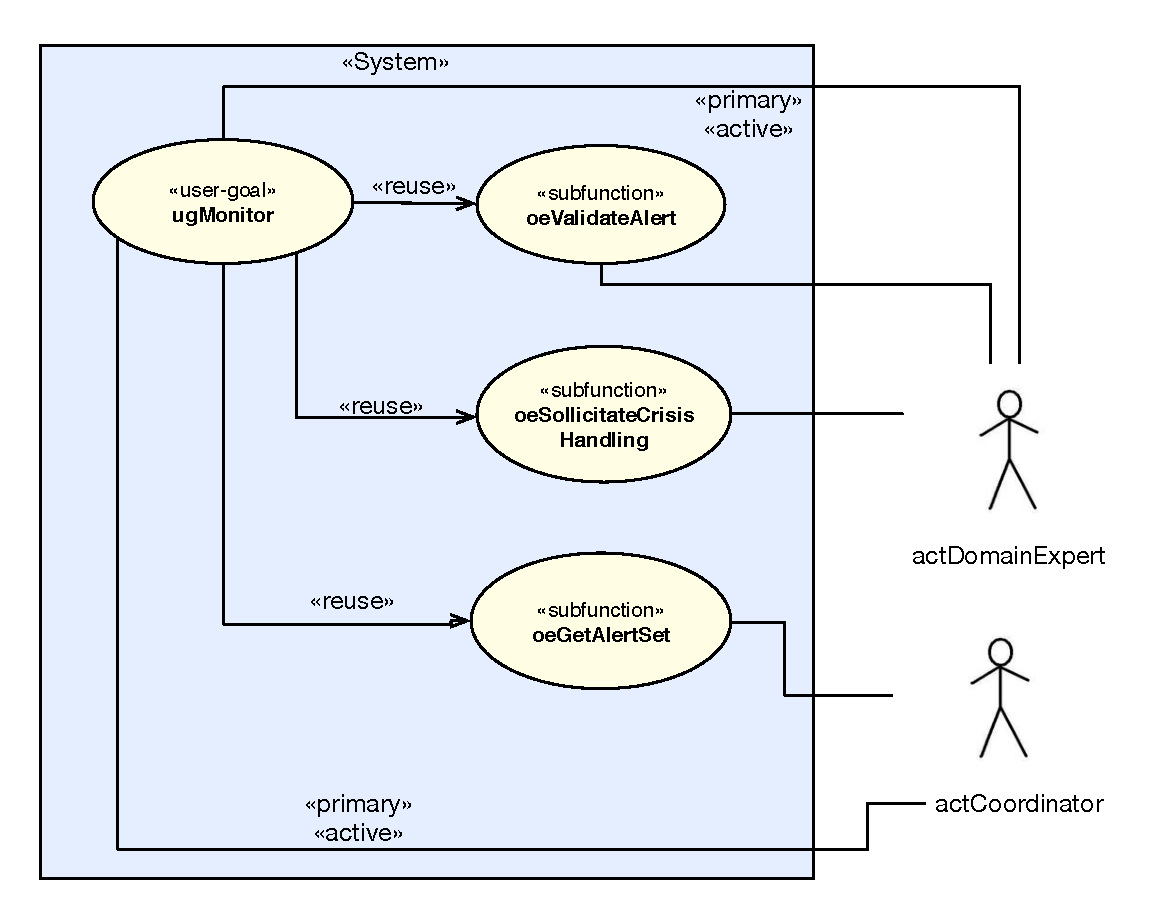
\includegraphics[width=180mm]{./images/UgMonitor.eps}\normalsize}
\end{center}
\caption[\msricrash Use Case Diagram: UgMonitor Diagram]{\msricrash Use Case Diagram: UgMonitor}
\label{fig:icrash-RE-UCD-UgMonitor}
\end{figure}
\vspace{0.5cm}

